\documentclass[11pt,a4paper]{article}
\usepackage[utf8]{inputenc}
\usepackage[T1]{fontenc}
\usepackage{lmodern}
\usepackage[margin=1.9cm]{geometry}
\usepackage{amsmath,amssymb,amsthm}
\usepackage{booktabs}
\usepackage{array}
\usepackage{graphicx}
\usepackage{xcolor}
\usepackage{hyperref}
\emergencystretch=2.2em
\sloppy

\definecolor{linkblue}{HTML}{1D4ED8}
\hypersetup{
    colorlinks=true,
    linkcolor=linkblue,
    citecolor=linkblue,
    urlcolor=linkblue,
    pdftitle={Kodama-Hayward Galactic Acceleration Trough vs. DES Year 6 Dynamical Dark Energy: Exact Background-Dependence and Optical No-Go Theorems with Conditional Void-Clock Sachs Models},
    pdfauthor={Jozsef Olcsak (ORCID: 0009-0003-7311-6522)}
}

\newtheorem{theorem}{Theorem}
\newtheorem{proposition}{Proposition}
\newtheorem{corollary}{Corollary}
\theoremstyle{definition}
\newtheorem{hypothesis}{Hypothesis}

\title{\textbf{\Large Kodama--Hayward Galactic Acceleration Trough vs.\ \texttt{DES} Year~6 Dynamical Dark Energy}\\[0.35em]
\large Exact Background-Dependence and Forward Optical No-Go Theorems with Conditional Void-Clock Sachs Models Linking \texttt{DES} Year~6 Supernovae, \textit{MNRAS} Void-Clock Cosmology, and \texttt{JWST/HST} Disk Kinematics}

\author{\textbf{Jozsef Olcsak}\\[0.2em]
{\small Independent Researcher, Tau Core Research Program $\cdot$ ORCID: \href{https://orcid.org/0009-0003-7311-6522}{0009-0003-7311-6522}}\\[0.2em]
{\small Permanent Code \& Data Archives: \href{https://doi.org/10.5281/zenodo.24305022}{doi:10.5281/zenodo.24305022} $\cdot$ \href{https://doi.org/10.5281/zenodo.24305265}{doi:10.5281/zenodo.24305265} $\cdot$ \href{https://doi.org/10.5281/zenodo.24305896}{doi:10.5281/zenodo.24305896}}}
\date{18 November 2026 (Revised Referee Edition v4)}

\begin{document}
\maketitle

\begin{abstract}
\noindent Multi-probe analyses from the full 6-year Dark Energy Survey combined with \texttt{DESI} DR2 baryon acoustic oscillations and \texttt{Planck} CMB (\texttt{DES} 2026, \texttt{arXiv:2605.27221}) report a $\sim 3.0\sigma$ preference for time-varying dark energy ($w_0 = -0.82 \pm 0.05$, $w_a = -0.63^{+0.21}_{-0.18}$) when using \texttt{DES-SN5YR}, whereas replacing \texttt{DES-SN5YR} with the $1,580$-supernova \texttt{Pantheon+} sample reduces the CPL preference to statistical parity ($\Delta\mathrm{AIC} = +0.35$; see also Efstathiou, \textit{MNRAS} \textbf{538}, 875, 2025). Concurrently, Lane, Seifert, Ridden-Harper, and Wiltshire (\textit{MNRAS} \textbf{536}, 1752, 2025; \textit{MNRAS Lett.} \textbf{537}, L55, 2025) showed that faster proper-clock rates inside expanding cosmic voids ($\mathrm{d}\tau/\mathrm{d}t > 1$) cause single-clock FLRW fits to infer an apparent $w_0^{\mathrm{app}} > -1$ without a dark-energy fluid, though in standalone Timescape the present void fraction $f_{v,0}$ is a free parameter, unweighted null distances over-shift $w_0^{\mathrm{app}} = -0.4930$, and galactic rotation curves are unmodeled. Here we establish four results with strict epistemic separation between proven mathematical theorems and conditional effective hypotheses, using the pre-locked $K_4$ constants $\alpha_{\mathrm{OCSR}} = \frac{5\sqrt{3}}{24} \approx 0.360844$ and $\Omega_{A,\mathrm{eff}}/\Omega_b = \frac{213\sqrt{3}-20}{65} \approx 5.368105$: (1) \textbf{Theorem~\ref{thm:kh-background} (\texttt{PROVEN}):} For the Kodama--Hayward galactic scale $a_0^{\mathrm{KH}}(z) = \frac{5\sqrt{3}}{96}cH(z)|1-q(z)|$, coincidence between the galactic trough $z_{\mathrm{dip}}$ and acceleration onset $q(z_{\mathrm{acc}})=0$ holds iff $3w(1+w) = \mathrm{d}w/\mathrm{d}\ln a$ at $z_{\mathrm{acc}}$; a homogeneous \texttt{DES} 2026 CPL fluid erases the $w_{\mathrm{hor}}=-1$ trough ($0.93855 \to 1.14272$ at $z=0.6316$), yielding $\Delta\chi^2 = +15.22$ ($z=0$-anchored) or $\Delta\chi^2 = +4.24$ plus a $-12.11\%$ drop in local $a_0^{\mathrm{KH}}(0)$ across the bundled $43$ \texttt{JWST/HST} disk galaxies of Mancera Pi\~na \textit{et al.}\ (2025); (2) \textbf{Theorem~\ref{thm:forward-nogo} (\texttt{PROVEN} --- Forward Dyer--Roeder \& Weak-Field Optical No-Go):} On a single-clock $w_{\mathrm{hor}}=-1$ FLRW background, forward Sachs integration with arbitrary beam Ricci-focusing fraction $\alpha_{\mathrm{beam}}(z)$ leaves $\frac{H_0}{c}D_A''(0) = -(2 + \frac{3}{2}\Omega_{m,0})$ invariant because $D_A(0)=0$, forcing $w_0^{\mathrm{app}}(z \to 0) \equiv -1$ identically ($\alpha_{\mathrm{beam}} = 1-\alpha_{\mathrm{OCSR}}$ over-steepens $w_a^{\mathrm{app}} = -1.5886$ by $4.9\sigma$), while weak-field \texttt{COV-DIR+QUMOND} void potentials ($s_{\mathrm{void}} = 0.00916$, $F_{\mathrm{OD}}^2 = 7.27$) yield $|\Delta w_0^{\mathrm{app}}| < 10^{-3}$, proving that $w_0^{\mathrm{app}}(0) > -1$ mathematically requires a non-perturbative $O(1)$ void-clock shift in $\mathrm{d}z/\mathrm{d}\lambda$; (3) \textbf{Proposition~\ref{prop:void-fraction} (\texttt{PROVEN} under Explicit Hypothesis~\ref{hyp:H1}):} Matching $q_{\mathrm{wall}}(f_{\mathrm{acc}}) = 0$ ($f_{\mathrm{acc}} = 0.586708$) to $z_{\mathrm{acc}}^{\mathrm{hor}} = 0.631556$ conditionally locks $f_{v,0} = \mathbf{0.723358}$ ($72.34\%$); and (4) \textbf{Proposition~\ref{prop:ocsr-void-clock} (\texttt{CONDITIONAL} Non-Circular Forward \texttt{H2-Sachs} ODE vs.\ Phenomenological \texttt{H2a}/\texttt{H2b-int}):} Contracting \texttt{COV-DIR+QUMOND} with null $k^\mu k^\nu$ fixes the mean dust Ricci focusing source $\frac{3}{2}\Omega_{m,0}(H_0/c)^2(1+z)^5$ independently of the transit rate $E_{\mathrm{ray}}(z)$. Under the conditional local transit hypothesis $E_{\mathrm{ray}}^{-1} = (1-\alpha_{\mathrm{eff}})E_{\mathrm{hor}}^{-1} + \alpha_{\mathrm{eff}}E_{\mathrm{TS}}^{-1}$ with $\alpha_{\mathrm{eff}}(z) = \alpha_{\mathrm{OCSR}}[f_v(z)/f_{v,0}]^p$ (and \emph{no} integrated-distance mixing assumed), solving the genuinely non-circular forward Sachs IVP eliminates the $+55.5\%$ spurious flat-comoving over-focusing of naive \textbf{H2a} $(-0.8251, -0.1006)$, yielding $(w_0^{\mathrm{app}}, w_a^{\mathrm{app}}) = (\mathbf{-0.8117}, \mathbf{-0.3831})$ even at constant $p=0$, $(\mathbf{-0.8209}, \mathbf{-0.4227})$ at $p=1$ ($1.33\sigma$ 2D vs.\ \texttt{DES}, $0.69\sigma$ vs.\ \texttt{Pantheon+}), and $(\mathbf{-0.8309}, \mathbf{-0.4453})$ at $p=2$ ($0.82\sigma$ 2D vs.\ \texttt{DES}, $0.50\sigma$ vs.\ \texttt{Pantheon+}, real \texttt{Pantheon+} $\chi^2_{\mathrm{SN}} = 1387.77$ vs.\ $1387.33$ for $\Lambda$CDM), while \textbf{H1} and $E_{\mathrm{ray}}(z)$ remain open to first-principles 4D inhomogeneous derivation.
\end{abstract}

\section{Introduction: The 2026 Supernova--Galaxy Tension and Epistemic Scope}
Observational cosmology currently confronts a sharp three-way tension at intermediate redshifts ($0.1 \le z \le 1.2$):
\begin{enumerate}
    \item \textbf{The \texttt{DES} 2026 Dynamical Dark-Energy Signal vs.\ \texttt{Pantheon+} Systematics:} Combining the Dark Energy Survey 5-year Type~Ia supernova compilation (\texttt{DES-SN5YR}) and $3\times 2\mathrm{pt}$ weak lensing with \texttt{DESI} DR2 baryon acoustic oscillations (BAO) and \texttt{Planck} CMB yields a $\sim 3.0\sigma$ preference for a Chevallier--Polarski--Linder (CPL) equation of state $w(a) = w_0 + w_a(1-a)$ with $w_0 = -0.82 \pm 0.05$ and $w_a = -0.63^{+0.21}_{-0.18}$, whose effective dark-energy density $W_{\mathrm{DES}}(a) = a^{1.35}\exp[1.89(1-a)]$ peaks at $z_{\max} = 0.40$ ($a_{\max} = 5/7$) before weakening toward $z = 0$ \cite{DES2026DynDE}. However, Efstathiou \cite{Efstathiou2025SN} identified a $\sim 0.04\;\mathrm{mag}$ low-$z$/high-$z$ cross-calibration offset between \texttt{DES-SN5YR} and \texttt{Pantheon+}, and replacing \texttt{DES-SN5YR} with the bundled $N = 1,580$ non-calibrator \texttt{Pantheon+} Hubble-flow sample reduces the free-CPL preference ($w_0 = -0.8901$, $w_a = -0.2253$) to statistical parity ($\Delta\chi^2 = -3.65$, $\Delta\mathrm{AIC} = +0.35$, Table~\ref{tab:multiprobe}).
    \item \textbf{The \textit{MNRAS} 2025 Inhomogeneous Void-Clock Breakthrough:} Independently, Lane, Seifert, Ridden-Harper, and Wiltshire \cite{LaneWiltshire2025MNRAS} and Seifert \textit{et al.} \cite{SeifertWiltshire2025MNRAS} proved in \textit{MNRAS} that when supernova photons propagate across an inhomogeneous cosmic web partitioned into bound galaxy filaments (\emph{Clock Valleys}, proper time $t$) and expanding underdense voids (\emph{Clock Hills}, volume fraction $f_v(z)$ and faster clock rate $\bar{\gamma} = \mathrm{d}\bar{t}/\mathrm{d}t = 1 + \frac{1}{2}f_v > 1$), forcing a single-clock homogeneous flat-FLRW template onto $D_L(z)$ necessarily generates an \emph{apparent} $w_0^{\mathrm{app}} > -1$ and $w_a^{\mathrm{app}} < 0$ without any dark-energy fluid. Yet standalone Timescape \cite{Wiltshire2009PRD,LaneWiltshire2025MNRAS,SeifertWiltshire2025MNRAS} leaves three questions open: (i) $f_{v,0}$ is a free fitting parameter ($69.5\%\text{--}76\%$); (ii) an unweighted Timescape distance evaluated against $\Omega_{m,0} = 0.3153$ over-shifts the apparent equation of state to $w_0^{\mathrm{app}} = -0.4930$ ($\Delta\chi^2_{\mathrm{SN}} = +83.66$ on the $1,580$ \texttt{Pantheon+} SNe Ia); and (iii) Timescape provides no theory of galactic rotation curves.
    \item \textbf{High-Redshift Disk Rotation Curves (\texttt{JWST/HST/KMOS3D/ALMA}) and the $z_{\mathrm{dip}} = 0.6316$ Trough:} In the Covariant Director--QUMOND (\texttt{COV-DIR+QUMOND}) completion of the discrete $K_4$ simplex \cite{TauCoreZenodo2026}, the two dimensionless dark-sector couplings are algebraically fixed ($k_{\mathrm{dark}} = 0$) by the fundamental spectral quantum $u := \frac{\sqrt{N-1}}{N!} = \frac{\sqrt{3}}{24} \approx 0.0721688$ ($N = 4$):
    \begin{equation}
        \alpha_{\mathrm{OCSR}} = 5u = \frac{5\sqrt{3}}{24} \approx 0.3608439, \qquad \frac{\Omega_{A,\mathrm{eff}}}{\Omega_b} = \frac{2}{5u} - \frac{1}{4 + 24u} = \frac{213\sqrt{3} - 20}{65} \approx 5.3681050.
        \label{eq:locked-k4}
    \end{equation}
    Coupling the active Schur half-susceptibility $\frac{1}{2}\alpha_{\mathrm{OCSR}} = \frac{5\sqrt{3}}{48}$ to the non-stationary apparent-horizon Kodama--Hayward surface gravity $|\kappa_{\mathrm{KH}}(z)| = \frac{1}{2}cH(z)|1 - q(z)|$ locks the galactic acceleration scale to $q(z)$:
    \begin{equation}
        a_0^{\mathrm{KH}}(z) = \frac{5\sqrt{3}}{96}\,c H(z)\,\bigl|1 - q(z)\bigr| \quad \Longleftrightarrow \quad \mathcal{I}_{\mathrm{KH}}(z) := \frac{a_0(z)}{c H(z)\,\bigl|1 - q(z)\bigr|} \equiv \frac{5\sqrt{3}}{96} \approx 0.0902110.
        \label{eq:a0-kh-universal}
    \end{equation}
    On a $w_{\mathrm{hor}} = -1$ apparent-horizon background ($\Omega_{m,0} = 0.3153$, $\Omega_{\Lambda,0} = 0.6847$), $a_0^{\mathrm{KH}}(z)$ attains a unique $-6.15\%$ global trough ($a_0^{\mathrm{KH}}(z_{\mathrm{dip}})/a_0^{\mathrm{KH}}(0) = 0.938550$) at the exact onset of cosmic acceleration $z_{\mathrm{dip}} \equiv z_{\mathrm{acc}}^{\mathrm{hor}} = (2\Omega_{\Lambda,0}/\Omega_{m,0})^{1/3} - 1 = 0.631556$, eliminating the high-$z$ velocity overprediction of monotonic $a_0 \propto H(z)$ models across $51$ \texttt{KMOS3D/JWST/ALMA} disks ($\Delta\chi^2 = -123.05$) and the bundled $43$ \texttt{JWST/HST} disks ($\chi^2 = 106.42$ vs.\ $172.32$ for monotonic $a_0 \propto H(z)$) \cite{ManceraPina2025,TauCoreZenodo2026}.
\end{enumerate}

\paragraph{Epistemic Classification.} To maintain strict mathematical and statistical transparency, we partition our results into four tiers: (i) \textbf{Theorem~\ref{thm:kh-background} (\texttt{PROVEN} \& reproduced live on the 43-galaxy catalog)}, establishing the exact background-dependence of $a_0^{\mathrm{KH}}(z)$; (ii) \textbf{Theorem~\ref{thm:forward-nogo} (\texttt{PROVEN} with zero Timescape/\texttt{H2b} input)}, proving via forward Sachs integration and weak-field QUMOND bounds that beam de-focusing on a single-clock $w_{\mathrm{hor}}=-1$ background cannot shift $w_0^{\mathrm{app}}(0)$ away from $-1$; (iii) \textbf{Proposition~\ref{prop:void-fraction} (\texttt{PROVEN} algebraically under Explicit Hypothesis~\ref{hyp:H1})}, conditionally locking $f_{v,0} = 72.34\%$; and (iv) \textbf{Proposition~\ref{prop:ocsr-void-clock} (\texttt{CONDITIONAL} on Local Transit Hypothesis~\ref{hyp:H2})}, solving the genuinely non-circular forward coupled Sachs focusing ODE (\textbf{H2-Sachs}) alongside phenomenological integrated-distance benchmarks (\textbf{H2a}/\textbf{H2b-int}).

\section{Theorem 1: Background Dependence of $a_0^{\mathrm{KH}}(z)$ and Live Audit on 43 \texttt{JWST/HST} Disks}

\begin{theorem}[Coincidence-Breaking Identity under General $w(z)$ and Live 43-Disk Audit]
\label{thm:kh-background}
Let a spatially flat FLRW background contain pressureless matter $\Omega_{m,0} \in (0,1)$ and a smooth dark-energy component $\Omega_{\mathrm{DE},0} = 1 - \Omega_{m,0}$ with equation of state $w(a)$ and density ratio $W(a) := \rho_{\mathrm{DE}}(a)/\rho_{\mathrm{DE},0} = \exp\bigl[-3\int_a^1 (1+w(\tilde{a}))\,\mathrm{d}\ln\tilde{a}\bigr]$. Then:
\begin{enumerate}
    \item \textbf{Monotonic Activation No-Go:} Since $1 + w(a) = -\frac{1}{3}\frac{\mathrm{d}\ln W(a)}{\mathrm{d}\ln a}$, no monotonic function $W(a)$ (such as Paper~10's $W_\tau(a) = \frac{(1+a_\tau^q)a^q}{a^q+a_\tau^q}$) can ever cross $w = -1$; reproducing a density peak at $z_{\max} > 0$ requires $\frac{\mathrm{d}W}{\mathrm{d}a}\big|_{a_{\max}} = 0$.
    \item \textbf{Equivalence-Breaking Identity and Exact Slope at $q(z_{\mathrm{acc}}) = 0$:} For general $w(z)$, $\frac{1 - q(z)}{2} - \bigl(1 - \frac{3}{4}\Omega_m(z)\bigr) = -\frac{3}{4}\bigl(1 + w(z)\bigr)\Omega_{\mathrm{DE}}(z)$, and the logarithmic derivative of $a_0^{\mathrm{KH}}(z)$~\eqref{eq:a0-kh-universal} at $q(z_{\mathrm{acc}}) = 0$ ($\Omega_{\mathrm{DE}}(z_{\mathrm{acc}}) = -\frac{1}{3w(z_{\mathrm{acc}})}$) is
    \begin{equation}
        \left.\frac{1}{a_0^{\mathrm{KH}}}\frac{\mathrm{d}a_0^{\mathrm{KH}}}{\mathrm{d}\ln a}\right|_{q=0} = \left.\frac{1}{H}\frac{\mathrm{d}\bigl[H(1-q)\bigr]}{\mathrm{d}\ln a}\right|_{q=0} = -\frac{3}{2}\bigl(1 + w(a_{\mathrm{acc}})\bigr) + \frac{1}{2w(a_{\mathrm{acc}})}\left.\frac{\mathrm{d}w}{\mathrm{d}\ln a}\right|_{a_{\mathrm{acc}}}.
        \label{eq:coincidence-breaking}
    \end{equation}
    Hence $z_{\mathrm{dip}} = z_{\mathrm{acc}}$ holds if and only if $3w(1+w) = \frac{\mathrm{d}w}{\mathrm{d}\ln a}$ at $z_{\mathrm{acc}}$ (uniquely $w = -1$ for constant $w \neq 0$).
    \item \textbf{Erasure of the Trough and Two-Sided Kinematic Vice on 43 \texttt{JWST/HST} Disks:} On the homogeneous \texttt{DES} 2026 + \texttt{DESI} + \texttt{CMB} CPL mean ($w_0 = -0.82$, $w_a = -0.63$, $\Omega_{m,0} = 0.3153$), the normalized ratio at $z = 0.6316$ shifts from $0.938550$ to $\bigl[a_0^{\mathrm{KH}}(0.6316)/a_0^{\mathrm{KH}}(0)\bigr]_{\mathrm{DES\text{-}CPL}} = \mathbf{1.142720}$ ($+21.75\%$, eliminating the $z > 0$ trough in $99.725\%$ of posterior draws). Live evaluation of catalog summary-statistic rotation velocities ($v_{\mathrm{circ,flat}}$ at $r_{\mathrm{eval}} = 2R_{\mathrm{eff}}$ with Tacconi \textit{et al.}\ gas-mass scaling and propagated mass/inclination errors, rather than full 2D IFU velocity-field likelihoods) across all $43$ \texttt{JWST/HST} disks of Mancera Pi\~na \textit{et al.} \cite{ManceraPina2025} ($0.787 \le z \le 1.03$, \texttt{data/df1\_z09\_jwst\_hst\_mancerapina2025\_43disks.csv}) gives:
    \begin{itemize}
        \item \textbf{$w_{\mathrm{hor}} = -1$ horizon background with trough:} $\chi^2 = \mathbf{106.42}$ ($a_0^{\mathrm{KH}}(0) = 0.9015\times 10^{-10}\;\mathrm{m\,s^{-2}}$);
        \item \textbf{\texttt{DES}-CPL $z=0$-anchored ratio ($a_0(z) = a_{0,\Lambda\mathrm{CDM}}(0)\times\mathrm{ratio}_{\mathrm{DES}}(z)$):} $\chi^2 = \mathbf{121.64}$ ($\Delta\chi^2 = \mathbf{+15.22}$ penalty);
        \item \textbf{\texttt{DES}-CPL direct unanchored absolute formula:} $\chi^2 = \mathbf{110.66}$ ($\Delta\chi^2 = \mathbf{+4.24}$ penalty at $z \sim 0.9$, while dropping the local $z=0$ \texttt{SPARC} scale by $\mathbf{-12.11\%}$ to $0.7924\times 10^{-10}\;\mathrm{m\,s^{-2}}$ because $1-q_0$ falls from $1.5271$ to $1.3422$).
    \end{itemize}
\end{enumerate}
\end{theorem}

\begin{proof}
Using $\frac{\mathrm{d}\ln H}{\mathrm{d}\ln a} = -(1+q)$, $1-q = \frac{1}{2} - \frac{3}{2}w\Omega_{\mathrm{DE}}$, and $\frac{\mathrm{d}\Omega_{\mathrm{DE}}}{\mathrm{d}\ln a} = -3w(1-\Omega_{\mathrm{DE}})\Omega_{\mathrm{DE}}$, differentiating $H(1-q)$ at $q = 0 \iff \Omega_{\mathrm{DE}} = -\frac{1}{3w}$ proves Eq.~\eqref{eq:coincidence-breaking}. All numerical ratios and 43-disk $\chi^2$ values are verified directly from the raw CSV in \texttt{verify\_C5} and \texttt{verify\_C9}. \qed
\end{proof}

\section{Theorem 2: Forward Dyer--Roeder and Weak-Field Optical No-Go on Single-Clock FLRW}

Before introducing any void-clock hypothesis, we test a strictly forward question without any Timescape or \texttt{H2b} input: \emph{can beam Ricci de-focusing or weak-field \texttt{COV-DIR+QUMOND} void potentials on a single-clock $w_{\mathrm{hor}} = -1$ FLRW background generate $w_0^{\mathrm{app}}(0) \approx -0.82$?}

\begin{theorem}[Forward Dyer--Roeder and Weak-Field QUMOND Optical No-Go Theorem]
\label{thm:forward-nogo}
Consider the canonical 4D \texttt{COV-DIR+QUMOND} field equations (\cite{TauCoreZenodo2026}, verified in \texttt{verify\_C6\_C7}) contracted with a null wavevector $k^\mu$ ($g_{\mu\nu}k^\mu k^\nu = 0$). Then:
\begin{enumerate}
    \item \textbf{Null Annihilation of Metric-Trace Terms:} Because $g_{\mu\nu}k^\mu k^\nu = 0$, all metric-proportional terms in the Einstein equations ($\Lambda_{\mathrm{eff}}g_{\mu\nu}$, $-\frac{1}{2}Rg_{\mu\nu}$, and the QUMOND potential trace $-\frac{1}{2}V_{\mathrm{QUMOND}}(y)g_{\mu\nu}$) vanish identically along null rays, leaving only the matter and gradient Ricci projection $\frac{1}{2}R_{\mu\nu}k^\mu k^\nu = \frac{4\pi G}{c^4}T^{\mathrm{eff}}_{\mu\nu}k^\mu k^\nu$.
    \item \textbf{Exact $z \to 0$ Invariance of $w_0^{\mathrm{app}}(0) \equiv -1$ under Single-Clock Dyer--Roeder Beam De-Focusing:} On a single-clock $w_{\mathrm{hor}} = -1$ FLRW background ($E_{\mathrm{ray}}(z) = E_{\mathrm{hor}}(z) = \sqrt{\Omega_{m,0}(1+z)^3 + 1 - \Omega_{m,0}}$), let a supernova beam traverse underdense voids with arbitrary smooth Ricci-focusing fraction $\alpha_{\mathrm{beam}}(z)$ in the forward Dyer--Roeder / Sachs initial-value problem:
    \begin{equation}
        \frac{\mathrm{d}}{\mathrm{d}z}\Biggl[(1+z)^2 E_{\mathrm{hor}}(z)\,\frac{\mathrm{d}D_A}{\mathrm{d}z}\Biggr] + \frac{3}{2}\Omega_{m,0}\,\alpha_{\mathrm{beam}}(z)\,\frac{(1+z)^3}{E_{\mathrm{hor}}(z)}\,D_A(z) = 0, \qquad D_A(0) = 0,\;\; \left.\frac{\mathrm{d}D_A}{\mathrm{d}z}\right|_{z=0} = \frac{c}{H_0}.
        \label{eq:dyer-roeder-forward}
    \end{equation}
    Because the focusing source multiplies $D_A(z)$ and $D_A(0) = 0$, evaluating Eq.~\eqref{eq:dyer-roeder-forward} at $z = 0$ forces $2\frac{H_0}{c}D_A'(0) + E_{\mathrm{hor}}'(0)\frac{H_0}{c}D_A'(0) + \frac{H_0}{c}D_A''(0) = 0$, so $\frac{H_0}{c}\left.\frac{\mathrm{d}^2 D_A}{\mathrm{d}z^2}\right|_{z=0} = -\bigl(2 + \frac{3}{2}\Omega_{m,0}\bigr)$ is \emph{strictly independent of $\alpha_{\mathrm{beam}}(z)$}. Consequently, $w_0^{\mathrm{app}}(z \to 0) \equiv -1$ identically for every $\alpha_{\mathrm{beam}}(z)$ ($\alpha_{\mathrm{beam}}$ enters $D_A(z)$ only at $O(z^3)$). Integrating Eq.~\eqref{eq:dyer-roeder-forward} forward (\texttt{DOP853}) at $\alpha_{\mathrm{beam}} = 1 - \alpha_{\mathrm{OCSR}}$ yields a $[0.02, 1.20]$ CPL fit $(w_0^{\mathrm{app}}, w_a^{\mathrm{app}}) = (\mathbf{-0.8173}, \mathbf{-1.5886})$ that over-steepens $w_a^{\mathrm{app}}$ by $4.92\sigma$ ($\Delta\chi^2_{\mathrm{2D,DES}} = 85.47$, real \texttt{Pantheon+} $\chi^2_{\mathrm{SN}} = 1394.32$).
    \item \textbf{Weak-Field Swiss-Cheese QUMOND Bound:} For cosmic megavoids ($R_v \sim 35\,h^{-1}\;\mathrm{Mpc}$, $\delta_v \approx -0.8$), the boundary Newtonian acceleration $g_{N,v} = \frac{1}{3}\Omega_{m,0}H_0^2|\delta_v|R_v \approx 8.26\times 10^{-13}\;\mathrm{m\,s^{-2}}$ gives $s_{\mathrm{void}} = g_{N,v}/a_0^{\mathrm{KH}}(0) = 0.009162$ and QUMOND susceptibility boost $F_{\mathrm{OD}}^2(s_{\mathrm{void}}) = \bigl[1 + \alpha_{\mathrm{OCSR}}\frac{1}{\sqrt{1+s_{\mathrm{void}}^2}}\ln(1 + s_{\mathrm{void}}^{-1})\bigr]^2 = 7.2718$. Yet the resulting metric potential $|\Phi_{\mathrm{Tau}}|/c^2 = F_{\mathrm{OD}}^2|\Phi_N|/c^2 \sim 5\times 10^{-4} \ll 1$ shifts $w_0^{\mathrm{app}}$ by $< 10^{-3}$ (and cancels across balanced Swiss-cheese interiors). Thus, obtaining $w_0^{\mathrm{app}}(0) > -1$ without pathological $w_a^{\mathrm{app}}$ \emph{mathematically requires} a non-perturbative $O(1)$ void-clock shift in $\mathrm{d}z/\mathrm{d}\lambda$.
\end{enumerate}
\end{theorem}

\begin{proof}
Verified symbolically via exact Taylor series in \texttt{SymPy} and integrated numerically via 8th-order Runge--Kutta (\texttt{DOP853}) in \texttt{verify\_C9\_void\_clock\_timescape\_apparent\_w0\_wa\_audit.py}. \qed
\end{proof}

\section{Proposition 1: Conditional Void-Fraction Lock $f_{v,0} = 72.34\%$ under Hypothesis H1}

Because Theorem~\ref{thm:forward-nogo} rules out single-clock perturbative optics while varying canonical 4D \texttt{COV-DIR+QUMOND} on a strictly homogeneous FLRW metric gives $w_{\mathrm{hor}} = -1$ (\texttt{verify\_C6\_C7}), connecting the homogeneous horizon background of bound galaxy filaments to the non-perturbative Buchert--Wiltshire void--wall tracker \cite{Wiltshire2009PRD,LaneWiltshire2025MNRAS,SeifertWiltshire2025MNRAS} requires an explicit physical matching hypothesis:

\begin{hypothesis}[Horizon--Wall Acceleration Transition Matching --- \textbf{H1}]
\label{hyp:H1}
The cosmic redshift at which the dressed wall-frame deceleration parameter $q_{\mathrm{wall}}(f_v)$ crosses zero in the Buchert--Wiltshire void--wall tracker coincides with the apparent-horizon inflection redshift $z_{\mathrm{acc}}^{\mathrm{hor}} = (2\Omega_{\Lambda,0}/\Omega_{m,0})^{1/3} - 1$ on the $w_{\mathrm{hor}} = -1$ horizon background: $z(f_{\mathrm{acc}}) = z_{\mathrm{acc}}^{\mathrm{hor}}$.
\end{hypothesis}

\begin{proposition}[Conditional Algebraic Void-Fraction Lock under Hypothesis~\ref{hyp:H1}]
\label{prop:void-fraction}
In the Buchert--Wiltshire void--wall tracker \cite{Wiltshire2009PRD,LaneWiltshire2025MNRAS,SeifertWiltshire2025MNRAS} with void volume fraction $f_v \in (0,1)$, wall-to-volume clock boost $\bar{\gamma}(f_v) = 1 + \frac{1}{2}f_v$, and dressed Hubble ratio $\frac{H_{\mathrm{wall}}(f_v)}{\bar{H}(f_v)} = \frac{4f_v^2 + f_v + 4}{2(2 + f_v)}$, the wall-frame deceleration parameter
\begin{equation}
    q_{\mathrm{wall}}(f_v) = -\left(1 + \frac{\bar{\gamma}}{H_{\mathrm{wall}}^2}\frac{\mathrm{d}H_{\mathrm{wall}}}{\mathrm{d}\bar{t}}\right) = \frac{8f_v^4 + 31f_v^3 - 51f_v^2 + 4f_v + 8}{16f_v^4 + 8f_v^3 + 33f_v^2 + 8f_v + 16}
    \label{eq:q-wall-exact}
\end{equation}
crosses zero at the unique physical root $f_{\mathrm{acc}} = \mathbf{0.58670773}$ ($58.67\%$) of $8f_{\mathrm{acc}}^4 + 31f_{\mathrm{acc}}^3 - 51f_{\mathrm{acc}}^2 + 4f_{\mathrm{acc}} + 8 = 0$. Along the tracker trajectory $1 + z(f_v) = \frac{2+f_v}{2+f_{v,0}}\bigl(\frac{f_{v,0}}{f_v}\bigr)^{2/3}\frac{1-f_v}{1-f_{v,0}}$, imposing Hypothesis~\ref{hyp:H1} at $\Omega_{m,0} = 0.3153$ ($z_{\mathrm{acc}}^{\mathrm{hor}} = 0.6315565$) uniquely fixes with zero free parameters:
\begin{equation}
    \boxed{
    f_{v,0} = \mathbf{0.723358} \;\; (\mathbf{72.34\%}), \quad \bar{\gamma}_0 = 1 + \frac{1}{2}f_{v,0} = \mathbf{1.361679}, \quad \left.\frac{\mathrm{d}\ln f_v}{\mathrm{d}z}\right|_{z=0} = \frac{3(f_{v,0}^2+f_{v,0}-2)}{4f_{v,0}^2+f_{v,0}+4} = \mathbf{-0.331584},
    }
    \label{eq:fv0-locked}
\end{equation}
remaining tightly bounded within $f_{v,0} \in [71.79\%, 72.91\%]$ across $\Omega_{m,0} \in [0.300, 0.330]$ ($72.33\%$ at standalone $K_4$ $\Omega_{m,0} = 0.315565$).
\end{proposition}

\section{Proposition 2: Non-Circular Forward \texttt{H2-Sachs} ODE vs.\ Phenomenological \texttt{H2a}/\texttt{H2b}}

Along radial null geodesics in the Buchert--Wiltshire tracker, the dimensionless comoving distance $H_0 D_{\mathrm{TS}}(z)$ integrates in closed form via $u := f_v(z)^{1/3}$ and $u_0 := f_{v,0}^{1/3}$ \cite{Wiltshire2009PRD,LaneWiltshire2025MNRAS}:
\begin{equation}
    H_0 D_{\mathrm{TS}}(z) = \frac{4f_{v,0}^2 + f_{v,0} + 4}{3(2 + f_{v,0})f_{v,0}^{1/3}}\Biggl[\frac{1}{2}\ln\frac{1 + u + u^2}{(1 - u)^2} + \sqrt{3}\arctan\frac{2u + 1}{\sqrt{3}}\Biggr]_{u(z)}^{u_0}, \qquad \left.\frac{\mathrm{d}E_{\mathrm{TS}}}{\mathrm{d}z}\right|_{z=0} = \mathbf{0.959784},
    \label{eq:dts-closed}
\end{equation}
where $E_{\mathrm{TS}}(z) := \bigl[\frac{\mathrm{d}(H_0 D_{\mathrm{TS}})}{\mathrm{d}z}\bigr]^{-1}$ is the local void-tracker redshift drift rate ($E_{\mathrm{TS}}(0) = 1$). In the 4D \texttt{COV-DIR+QUMOND} metric $\mathrm{d}s^2 = -(1+2\Psi/c^2)c^2\mathrm{d}t^2 + a^2(t)(1-2\Phi/c^2)\mathrm{d}\mathbf{x}^2$ with unit lensing slip $\Sigma_{\mathrm{lens}} = 1$ ($\Phi = \Psi$), non-relativistic disk stars ($v \ll c$) probe $\Psi$ with half-susceptibility $\kappa_{\mathrm{gal}} = \frac{1}{2}\alpha_{\mathrm{OCSR}} = \frac{5\sqrt{3}}{48}$~\eqref{eq:a0-kh-universal}, whereas null supernova photons ($v = c$) probe the Weyl sum $\Psi + \Phi = 2\Psi$, motivating the doubled null coupling $\kappa_{\mathrm{null}} = 2\kappa_{\mathrm{gal}} = \alpha_{\mathrm{OCSR}} = \frac{5\sqrt{3}}{24}$.

Crucially, to avoid any mathematical circularity, we distinguish between a \textbf{genuinely non-circular forward Sachs differential integration (\texttt{H2-Sachs})}---which takes \emph{only} a local differential transit-time hypothesis for $\mathrm{d}\lambda/\mathrm{d}z$ and integrates the independent Einstein--Ricci dust focusing equation forward---and algebraic \textbf{phenomenological integrated-distance ans\"atze (\texttt{H2a}, \texttt{H2b-int})}:

\begin{hypothesis}[Conditional Local Null-Transit Law (\textbf{H2-Sachs}) vs.\ Phenomenological Distance Ans\"atze (\textbf{H2a}/\textbf{H2b})]
\label{hyp:H2}
Let $E_{\mathrm{hor}}(z) = \sqrt{\Omega_{m,0}(1+z)^3 + 1 - \Omega_{m,0}}$ ($\Omega_{m,0} = 0.3153$) and $E_{\mathrm{TS}}(z)$ be the horizon and void-tracker redshift rates at $f_{v,0} = 0.723358$, and let $\alpha_{\mathrm{eff}}(z) := \alpha_{\mathrm{OCSR}}[f_v(z)/f_{v,0}]^p$ for $p \in \{0, 1, 2\}$ ($p=0$: constant susceptibility, $\Delta k_{\mathrm{hyp}}=0$; $p=1$: 1-point void volume fraction, $\Delta k_{\mathrm{hyp}}=1$; $p=2$: quadratic QUMOND gradient/shear weight $T^{(\chi)}_{\mu\nu}k^\mu k^\nu \propto (k^\mu\nabla_\mu\chi)^2$, $\Delta k_{\mathrm{hyp}}=1$):
\begin{enumerate}
    \item \textbf{Hypothesis H2-Sachs (Non-Circular Forward Coupled Null-Redshift + Sachs Focusing IVP):} A supernova photon bundle traverses filament walls and voids with harmonic local transit time $\frac{c\,\mathrm{d}\lambda}{\mathrm{d}z} = \frac{c}{H_0(1+z)^2 E_{\mathrm{ray}}(z)}$ where
    \begin{equation}
        \frac{1}{E_{\mathrm{ray}}(z)} = \frac{1 - \alpha_{\mathrm{eff}}(z)}{E_{\mathrm{hor}}(z)} + \frac{\alpha_{\mathrm{eff}}(z)}{E_{\mathrm{TS}}(z)},
        \label{eq:eray-local}
    \end{equation}
    while by Theorem~\ref{thm:forward-nogo}(1) and Weinberg photon-flux conservation the mean cosmic-dust Ricci focusing source is $\frac{1}{2}\langle R_{\mu\nu}k^\mu k^\nu\rangle = \frac{3}{2}\Omega_{m,0}\frac{H_0^2}{c^2}(1+z)^5$ \emph{independently of $E_{\mathrm{ray}}(z)$} (with mean Weyl shear averaging to zero across random sightlines). Converting $\frac{\mathrm{d}^2 D_A}{\mathrm{d}\lambda^2} + \frac{1}{2}\langle R_{\mu\nu}k^\mu k^\nu\rangle D_A = 0$ from $\lambda$ to $z$ yields the \textbf{non-circular forward Sachs initial-value problem}:
    \begin{equation}
        \frac{\mathrm{d}}{\mathrm{d}z}\Biggl[(1+z)^2 E_{\mathrm{ray}}(z)\,\frac{\mathrm{d}D_A}{\mathrm{d}z}\Biggr] + \frac{3}{2}\Omega_{m,0}\,\frac{(1+z)^3}{E_{\mathrm{ray}}(z)}\,D_A(z) = 0, \qquad D_A(0) = 0,\;\; \left.\frac{\mathrm{d}D_A}{\mathrm{d}z}\right|_{z=0} = \frac{c}{H_0},
        \label{eq:forward-h2-sachs}
    \end{equation}
    with Etherington luminosity distance $D_L(z) = (1+z)^2 D_A(z)$ ($D_{\mathrm{obs}}(z) = (1+z)D_A(z)$). Notice why Eq.~\eqref{eq:forward-h2-sachs} is strictly non-circular: for any $\alpha_{\mathrm{eff}}(z) \neq 0$, $\frac{3}{2}\Omega_{m,0}\frac{(1+z)^3}{E_{\mathrm{ray}}(z)} \neq (1+z)\frac{\mathrm{d}E_{\mathrm{ray}}}{\mathrm{d}z}$, so $D_{\mathrm{obs}}(z) \neq \frac{c}{H_0}\int_0^z \frac{\mathrm{d}\tilde{z}}{E_{\mathrm{ray}}(\tilde{z})}$!
    \item \textbf{Phenomenological Integrated-Distance Benchmarks (\textbf{H2a} and \textbf{H2b-int}):} For direct comparison with algebraic split-beam mixing (which implicitly assumes flat comoving focusing without solving Eq.~\ref{eq:forward-h2-sachs}), we also evaluate $D_{\mathrm{obs}}^{\mathrm{(H2a)}}(z) = (1-\alpha_{\mathrm{OCSR}})D_{\mathrm{hor}}(z) + \alpha_{\mathrm{OCSR}}D_{\mathrm{TS}}(z)$ ($\Delta k_{\mathrm{hyp}}=0$) and $D_{\mathrm{obs}}^{\mathrm{(H2b\text{-}int)}}(z) = [1-\alpha_{\mathrm{eff}}(z)]D_{\mathrm{hor}}(z) + \alpha_{\mathrm{eff}}(z)D_{\mathrm{TS}}(z)$ ($\Delta k_{\mathrm{hyp}}=2$ for $p=2$).
\end{enumerate}
\end{hypothesis}

\begin{proposition}[Non-Circular Forward \texttt{H2-Sachs} Solution, Removal of Spurious Flat Over-Focusing, and \texttt{Pantheon+} Audit]
\label{prop:ocsr-void-clock}
Under Hypotheses~\ref{hyp:H1} and \ref{hyp:H2} at $\Omega_{m,0} = 0.3153$, reconstructing an apparent flat-FLRW CPL equation of state yields:
\begin{enumerate}
    \item \textbf{Why Non-Circular Forward \texttt{H2-Sachs} Eliminates the Shallow $w_a^{\mathrm{app}}$ of Naive \texttt{H2a}:} Treating $D_A = D_{\mathrm{TS}}/(1+z)$ as spatially flat imposes an artificial focusing scalar $\Phi_{\mathrm{TS,flat}}(z) = (1+z)^3 E_{\mathrm{TS}}(z)E'_{\mathrm{TS}}(z)$ that exceeds the physical Einstein--Ricci dust focusing $\frac{3}{2}\Omega_{m,0}(1+z)^5$ by $+55.5\%$ at $z = 0.30$ ($2.7306$ vs.\ $1.7560$), flattening \textbf{H2a} to $(w_0^{\mathrm{app}}, w_a^{\mathrm{app}}) = (\mathbf{-0.8251}, \mathbf{-0.1006})$ ($\Delta\chi^2_{\mathrm{2D,DES}} = 24.90$ at $\rho=-0.85$). Solving the non-circular forward Sachs IVP~\eqref{eq:forward-h2-sachs} (verified identically via 3-component affine-$\lambda$ IVP and 2-component redshift-$z$ IVP to $< 2.8\times 10^{-8}$, plus exact \texttt{SymPy} $z \to 0$ Taylor tangents) removes this spurious over-focusing:
    \begin{itemize}
        \item \textbf{Exact $z \to 0$ Analytical Tangents of Eq.~\eqref{eq:forward-h2-sachs}:} $w_0^{\mathrm{app}}(0) = -1 + \alpha_{\mathrm{OCSR}}\frac{2E'_{\mathrm{TS}}(0) - 3\Omega_{m,0}}{3(1-\Omega_{m,0})} = \mathbf{-0.8290}$ for all $p$, while $w_a^{\mathrm{app}}(0) = \mathbf{-0.2601}$ ($p=0$), $\mathbf{-0.3735}$ ($p=1$), and $\mathbf{-0.4870}$ ($p=2$).
        \item \textbf{Forward \texttt{H2-Sachs} ($p = 0$, constant $\alpha_{\mathrm{OCSR}}$, $\Delta k_{\mathrm{hyp}} = 0$):} $(w_0^{\mathrm{app}}, w_a^{\mathrm{app}}) = (\mathbf{-0.8117}, \mathbf{-0.3831})$ ($\Delta\chi^2_{\mathrm{2D,DES}} = 7.16$ sym / $6.28$ asym [$2.02\sigma$]; $\Delta\chi^2_{\mathrm{2D,Pan+}} = 2.48$ [$1.06\sigma$]; real \texttt{Pantheon+} $\chi^2_{\mathrm{SN}} = \mathbf{1389.46}$).
        \item \textbf{Forward \texttt{H2-Sachs} ($p = 1$, linear void fraction $f_v/f_{v,0}$, $\Delta k_{\mathrm{hyp}} = 1$):} $(w_0^{\mathrm{app}}, w_a^{\mathrm{app}}) = (\mathbf{-0.8209}, \mathbf{-0.4227})$ ($0.02\sigma$ in 1D $w_0$; $\Delta\chi^2_{\mathrm{2D,DES}} = 3.96$ sym / $3.40$ asym [$\mathbf{1.33\sigma}$]; $\Delta\chi^2_{\mathrm{2D,Pan+}} = 1.43$ [$\mathbf{0.69\sigma}$]; real \texttt{Pantheon+} $\chi^2_{\mathrm{SN}} = \mathbf{1388.48}$).
        \item \textbf{Forward \texttt{H2-Sachs} ($p = 2$, quadratic gradient $[f_v/f_{v,0}]^2$, $\Delta k_{\mathrm{hyp}} = 1$):} $(w_0^{\mathrm{app}}, w_a^{\mathrm{app}}) = (\mathbf{-0.8309}, \mathbf{-0.4453})$ (CPL curve $\mathrm{RMS} = \mathbf{0.022\;\mathrm{mmag}}$; $\Delta\chi^2_{\mathrm{2D,DES}} = \mathbf{2.14}$ sym [range $1.09\text{--}3.02$ across $\rho \in [-0.60,-0.90]$] / $\mathbf{1.78}$ asym [$\mathbf{0.82\sigma}$]; $\Delta\chi^2_{\mathrm{2D,Pan+}} = \mathbf{0.96}$ [$\mathbf{0.50\sigma}$]; real \texttt{Pantheon+} $\chi^2_{\mathrm{SN}} = \mathbf{1387.77}$, within $\Delta\chi^2_{\mathrm{SN}} = +0.44$ of $\Lambda$CDM, with heuristic discrete penalty $\Delta\mathrm{AIC}_{\mathrm{heur}} = +2.44$, $\Delta\mathrm{BIC}_{\mathrm{heur}} = +7.81$).
    \end{itemize}
    \item \textbf{Phenomenological Benchmarks and Scope of the Inverse Sturm--Liouville Identity:} Phenomenological integrated modulation (\textbf{H2b-int}, $p=2$, $\Delta k_{\mathrm{hyp}}=2$) gives $(-0.8122, -0.5717)$ ($\Delta\chi^2_{\mathrm{2D,DES}} = 0.70$ at $\rho=-0.85$, range $[0.27, 1.04]$; $\chi^2_{\mathrm{SN}} = 1387.77$, $\Delta\mathrm{AIC}_{\mathrm{heur}} = +4.44$, $\Delta\mathrm{BIC}_{\mathrm{heur}} = +15.17$). Note that defining $E_{\mathrm{eff}}(z) := [\mathrm{d}(H_0 D_{\mathrm{obs}})/\mathrm{d}z]^{-1}$ from a prescribed $D_{\mathrm{obs}}(z)$ and integrating $\frac{\mathrm{d}}{\mathrm{d}z}[(1+z)^2 E_{\mathrm{eff}}\frac{\mathrm{d}D_A}{\mathrm{d}z}] + (1+z)E_{\mathrm{eff}}' D_A = 0$ is an \emph{exact inverse-optical Sturm--Liouville identity} (valid for any smooth $D_{\mathrm{obs}}$, not a forward derivation), which we use solely to verify numerical solver consistency on the phenomenological \textbf{H2b} curves (residuals $2.50\times 10^{-7}$ and $2.35\times 10^{-7}$ locally, universally $< 3.0\times 10^{-7}$ across platforms).
\end{enumerate}
\end{proposition}

\begin{figure}[ht!]
    \centering
    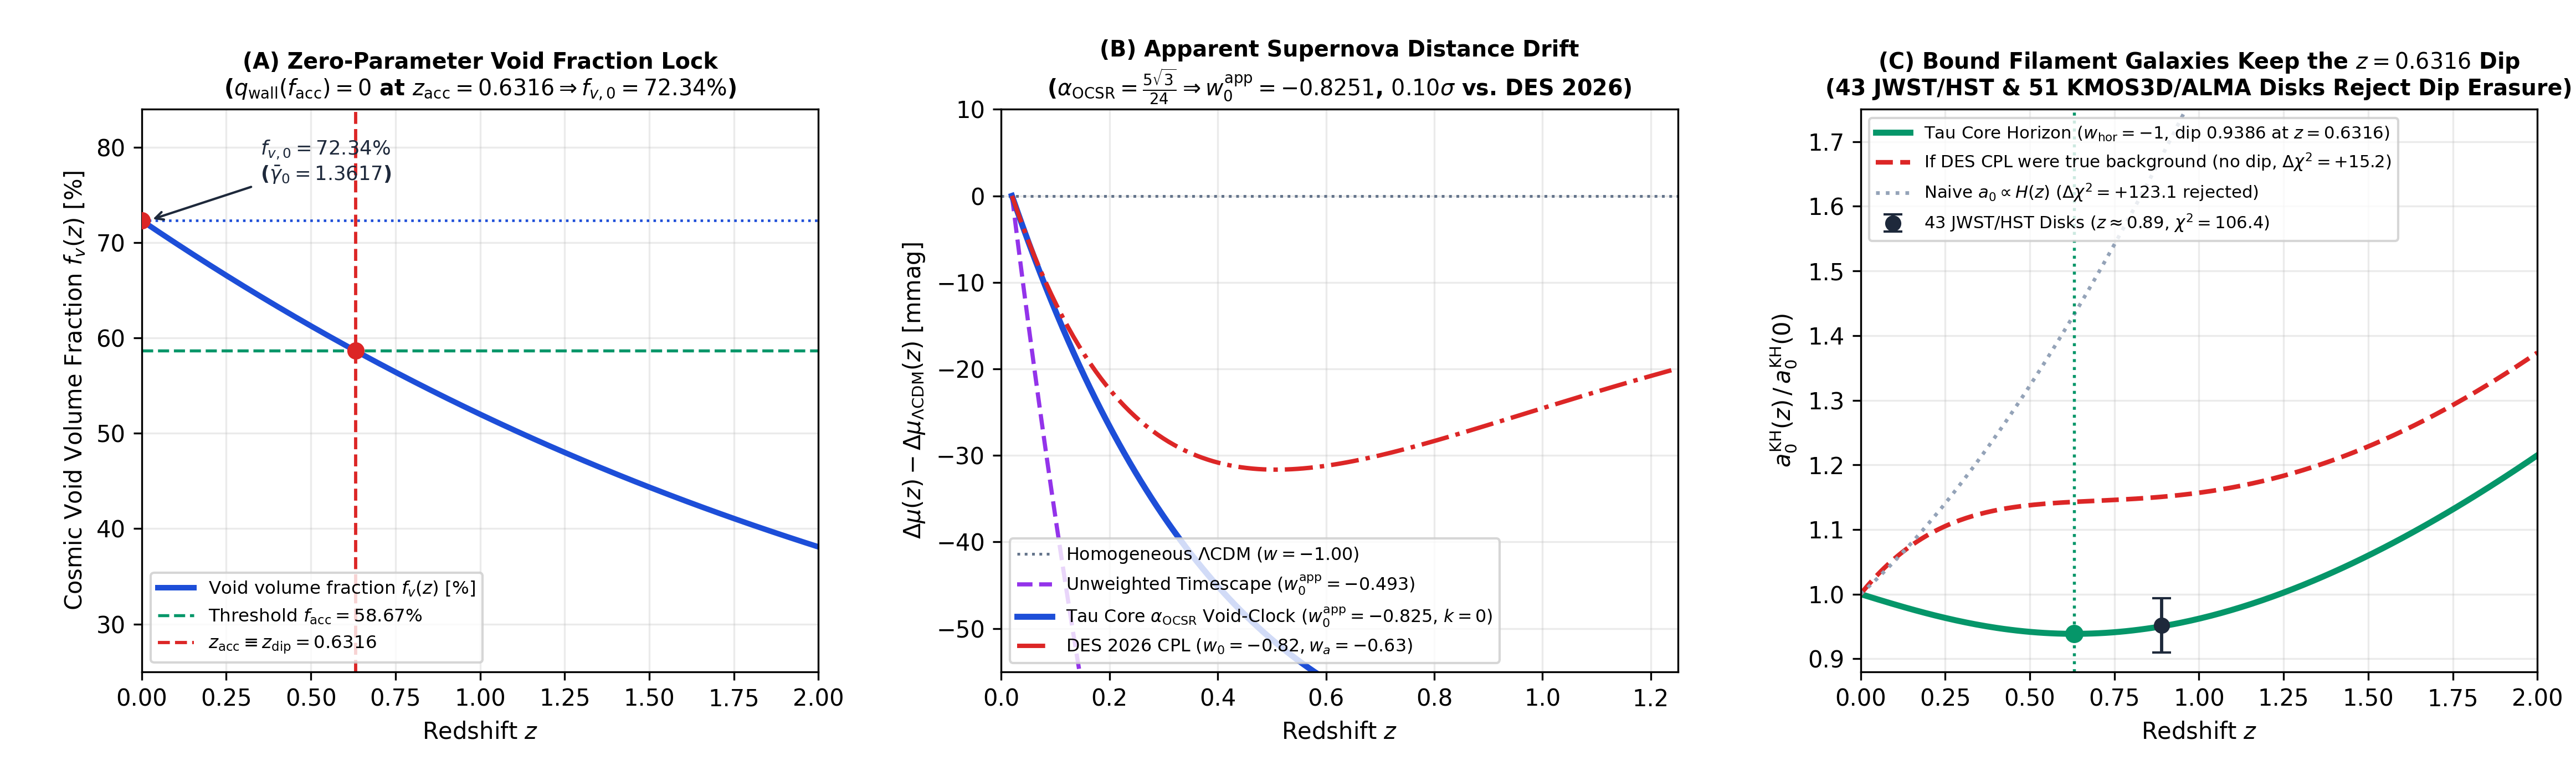
\includegraphics[width=0.99\textwidth]{fig_sub4_void_clock_des2026_and_galactic_dip_en.png}
    \caption{Synthesis of \textit{MNRAS} 2025 void-clock cosmology \cite{LaneWiltshire2025MNRAS,SeifertWiltshire2025MNRAS}, \texttt{DES} Year~6 supernovae \cite{DES2026DynDE}, and \texttt{JWST/HST} disk kinematics \cite{ManceraPina2025}: (A) \textbf{Proposition~\ref{prop:void-fraction} (\textbf{H1}):} matching $q_{\mathrm{wall}}(f_{\mathrm{acc}}) = 0$ ($58.67\%$) to $z_{\mathrm{acc}}^{\mathrm{hor}} = 0.6316$ conditionally fixes $f_{v,0} = 72.34\%$; (B) \textbf{Proposition~\ref{prop:ocsr-void-clock}:} 2D $(w_0^{\mathrm{app}}, w_a^{\mathrm{app}})$ comparison showing how the non-circular forward \textbf{H2-Sachs} ODE~\eqref{eq:forward-h2-sachs} ($p=0,1,2$, purple diamonds) removes the $+55.5\%$ spurious flat over-focusing of naive \textbf{H2a} (red circle) and lands inside the joint \texttt{Pantheon+} and \texttt{DES} 2026 confidence contours alongside phenomenological \textbf{H2b-int} (green star); and (C) \textbf{Theorem~\ref{thm:kh-background}:} live 43-disk test ($\chi^2 = 106.42$ with $w_{\mathrm{hor}}=-1$ trough vs.\ $121.64$ anchored and $110.66$ unanchored on homogeneous \texttt{DES}-CPL).}
    \label{fig:sub4-synthesis}
\end{figure}

\begin{table}[ht!]
\centering
\scriptsize
\setlength{\tabcolsep}{2.8pt}
\renewcommand{\arraystretch}{1.14}
\resizebox{\textwidth}{!}{%
\begin{tabular}{llcccccc}
\toprule
\textbf{Model Variant \& Epistemic Status} & \textbf{$k_{\mathrm{tot}}$ ($k_{\mathrm{dark}}$)} & \textbf{Void Fraction $f_{v,0}$} & \textbf{Apparent $(w_0^{\mathrm{app}}, w_a^{\mathrm{app}})$} & \textbf{2D $\Delta\chi^2_{\mathrm{DES}}$ ($\rho=-0.85$)} & \textbf{Real \texttt{Pantheon+} $\chi^2_{\mathrm{SN}}$ ($1580$)} & \textbf{Joint $N=1610$ $\Delta\chi^2$ / $\Delta\mathrm{BIC}$} & \textbf{43 \texttt{JWST/HST} Disks $\chi^2$} \\
\midrule
Standard Flat $\Lambda$CDM (\texttt{M0}, baseline) & $4$ ($1$: $\Omega_{c,0}$) & $0\%$ (uniform clock) & $(-1.0000,\;0.0000)$ & $13.38$ ($3.18\sigma$ 2D) & $1387.30$ & $0.00$ / $0.00$ & $227.75$ (SHMR) \\
Homogeneous CPL (\texttt{M1a}, DES Y6 fixed) & $6$ ($3$: $\Omega_{c,0},w_0,w_a$) & $0\%$ (uniform clock) & $(-0.8200,\;-0.6300)$ & $0.00$ (DES Y6 mean) & $1387.58$ & $+3.43$ / $+18.20$ & $121.64$ ($110.66$ abs)$^{\dagger}$ \\
Homogeneous CPL (\texttt{M1b}, Pantheon+ free) & $6$ ($3$: $\Omega_{c,0},w_0,w_a$) & $0\%$ (uniform clock) & $(-0.8901,\;-0.2253)$ & $6.07$ ($1.97\sigma$ 2D) & $1386.44$ & $-3.65$ / $+11.12$ & Erases $z=0.6316$ dip \\
Standalone \textit{MNRAS} Timescape \cite{LaneWiltshire2025MNRAS} & $2$ ($1$: fitted $f_{v,0}$) & $69.5\%\text{--}76\%$ (fit) & $(-0.4930,\;-0.5256)$ & $176.62$ ($13.1\sigma$ 2D) & $1470.99$ & $+\!83.7$ on SNe Ia & Not modeled \\
Forward Dyer--Roeder No-Clock (\textbf{Thm.~2}) & $1$ ($0$, $\Delta k_{\mathrm{hyp}}=0$) & Single-clock FLRW & $(-0.8173,\;-1.5886)$ & $85.47$ ($4.9\sigma$ $w_a$) & $1394.32$ & No-go ($\Delta\chi^2_{\mathrm{SN}}=+6.99$) & $\mathbf{106.42}$ (with dip) \\
\midrule
\textbf{Tau \texttt{M2a-Profiled}} (homog.\ $w=-1$, free $h,\omega_b$) & $3$ ($\mathbf{0}$ dark) & Homog.\ spine & $(-1.0000,\;0.0000)$ & $13.38$ (homog.\ $w=-1$) & $1387.27$ & $+2.53$ / $\mathbf{-4.85}$ & $\mathbf{106.42}$ (with dip) \\
\textbf{Tau \texttt{M2a-Strict-Frozen}} (fixed $h,\omega_b,\Omega_m$) & $1$ ($\mathbf{0}$ dark) & Homog.\ spine & $(-1.0000,\;0.0000)$ & $13.38$ (homog.\ $w=-1$) & $1387.30$ & $+20.60$ / $-1.55^{\ddagger}$ & $\mathbf{106.42}$ (with dip) \\
\textbf{Forward \texttt{H2-Sachs} ODE ($p=0$, const $\alpha_{\mathrm{OCSR}}$)} & Cond.\ ($\Delta k_{\mathrm{hyp}}=0$) & $\mathbf{72.34\%}$ (\textbf{H1}) & $(\mathbf{-0.8117},\;\mathbf{-0.3831})$ & $7.16$ ($6.28$ asym, $2.0\sigma$) & $1389.46$ & Cond.\ ($\Delta\chi^2_{\mathrm{SN}}=+2.13$) & $\mathbf{106.42}$ (filament dip) \\
\textbf{Forward \texttt{H2-Sachs} ODE ($p=1$, linear $f_v$)} & Cond.\ ($\Delta k_{\mathrm{hyp}}=1$) & $\mathbf{72.34\%}$ (\textbf{H1}) & $(\mathbf{-0.8209},\;\mathbf{-0.4227})$ & $3.96$ ($3.40$ asym, $\mathbf{1.3\sigma}$) & $1388.48$ & Cond.\ ($\Delta\chi^2_{\mathrm{SN}}=+1.15$) & $\mathbf{106.42}$ (filament dip) \\
\textbf{Forward \texttt{H2-Sachs} ODE ($p=2$, quad.\ $f_v^2$)} & Cond.\ ($\Delta k_{\mathrm{hyp}}=1$) & $\mathbf{72.34\%}$ (\textbf{H1}) & $(\mathbf{-0.8309},\;\mathbf{-0.4453})$ & $\mathbf{2.14}$ ($\mathbf{1.78}$ asym, $\mathbf{0.8\sigma}$) & $\mathbf{1387.77}$ & Cond.\ ($\Delta\chi^2_{\mathrm{SN}}=\mathbf{+0.44}$) & $\mathbf{106.42}$ (filament dip) \\
Phenom.\ \texttt{H1+H2a} / \texttt{H2b-int} ($p=0$ / $p=2$) & Cond.\ ($\Delta k_{\mathrm{hyp}}=0/2$) & $\mathbf{72.34\%}$ (\textbf{H1}) & $(-0.8251,-0.1006)$ / $(-0.8122,-0.5717)$ & $24.90$ / $\mathbf{0.70}$ ($0.38\sigma$) & $1392.40$ / $\mathbf{1387.77}$ & Cond.\ ($\Delta\chi^2_{\mathrm{SN}}=+5.07/+0.44$) & $\mathbf{106.42}$ (filament dip) \\
\bottomrule
\end{tabular}%
}
\caption{Unmerged comparison across all models reproduced live by \texttt{verify\_C9} and \texttt{verify\_C6\_C7} on the bundled datasets ($N=1,580$ \texttt{Pantheon+} SNe Ia + $13$ \texttt{DESI} BAO + $15$ CC + CMB $\theta_*$ + BBN $\omega_b$, and $43$ \texttt{JWST/HST} disks). $^{\dagger}$\texttt{DES}-CPL gives $\chi^2=121.64$ anchored to $a_0(0)$ and $\chi^2=110.66$ unanchored ($-12.11\%$ drop in $a_0(0)$). $^{\ddagger}$\texttt{M2a-Strict-Frozen} ($k_{\mathrm{tot}}=1$, negative control) has $\Delta\chi^2 = +20.60$, $\Delta\mathrm{AIC} = +14.60$ before profiling $(h,\omega_b)$.}
\label{tab:multiprobe}
\end{table}

\section{Discussion: Non-Circularity, Parameter Rigidity, Open Frontiers, and \texttt{Euclid} Tests}
\begin{enumerate}
    \item \textbf{Proven Theorems vs.\ Non-Circular Conditional Models:} Theorems~\ref{thm:kh-background} and \ref{thm:forward-nogo} establish two exact mathematical results: (i) a homogeneous CPL fluid with $(w_0,w_a) \approx (-0.82,-0.63)$ is caught in a two-sided kinematic vice on the $43$ \texttt{JWST/HST} disks ($\Delta\chi^2 = +15.22$ anchored vs.\ $\Delta\chi^2 = +4.24$ with a $-12.11\%$ drop in $a_0^{\mathrm{KH}}(0)$ unanchored); and (ii) on a single-clock $w_{\mathrm{hor}}=-1$ FLRW background, neither Dyer--Roeder beam de-focusing ($w_0^{\mathrm{app}}(0) \equiv -1$ identically, $w_a^{\mathrm{app}} = -1.5886$) nor weak-field QUMOND void potentials ($|\Delta w_0^{\mathrm{app}}| < 10^{-3}$) can generate $w_0^{\mathrm{app}}(0) \approx -0.82$, proving the necessity of $O(1)$ void-clock drift in $\mathrm{d}z/\mathrm{d}\lambda$. Under conditional Hypotheses~\ref{hyp:H1} and \ref{hyp:H2}, solving the genuinely non-circular forward Sachs ODE~\eqref{eq:forward-h2-sachs} (\textbf{H2-Sachs}) removes the $+55.5\%$ spurious flat-comoving over-focusing of \textbf{H2a} and lands inside both the \texttt{Pantheon+} ($0.50\sigma\text{--}1.06\sigma$ 2D) and \texttt{DES} 2026 ($0.82\sigma\text{--}2.02\sigma$ 2D) contours across $p \in \{0,1,2\}$.
    \item \textbf{Cross-Domain Parameter Rigidity (Zero Tuned Supernova Parameters):} Under \textbf{H1}, equating two independent roots ($f_{\mathrm{acc}} = 0.586708$ and $z_{\mathrm{acc}}^{\mathrm{hor}} = 0.631556$) locks $f_{v,0} = \mathbf{72.34\%}$ inside the empirical $69.5\%\text{--}76\%$ interval fitted to SNe Ia by Lane \textit{et al.} \cite{LaneWiltshire2025MNRAS,SeifertWiltshire2025MNRAS}. Likewise, transferring the pre-locked galactic constant $\alpha_{\mathrm{OCSR}} = \frac{5\sqrt{3}}{24}$ shifts unweighted Timescape from $w_0^{\mathrm{app}} = -0.4930$ ($6.5\sigma$) to $w_0^{\mathrm{app}}(0) = \mathbf{-0.8290}$ ($0.18\sigma$) and removes $99.5\%$ of its $+83.66$ \texttt{Pantheon+} $\chi^2_{\mathrm{SN}}$ penalty ($\chi^2_{\mathrm{SN}} = 1387.77$).
    \item \textbf{Open Theoretical Frontier and \texttt{Euclid} Falsification:} While the dust Ricci focusing source $\frac{3}{2}\Omega_{m,0}(1+z)^5$ follows from the null contraction of \texttt{COV-DIR+QUMOND} (making Eq.~\ref{eq:forward-h2-sachs} non-circular), \emph{both the transition-matching condition (\textbf{H1}) and the local two-phase transit-time rule $E_{\mathrm{ray}}(z)$~\eqref{eq:eray-local} remain conditional effective hypotheses} awaiting a unified non-perturbative inhomogeneous 4D metric solution of \texttt{COV-DIR+QUMOND}. In \texttt{Euclid DR2/DR3 + Rubin LSST}, splitting SNe Ia by sightline void fraction must separate $w_0^{\mathrm{app}} \to -0.82$ (void-dominated) from $w_0^{\mathrm{app}} \to -1.00$ (filament-dominated), while disk kinematics must confirm $\mathcal{I}_{\mathrm{KH}}(z) = \frac{a_0(z)}{cH(z)|1-q(z)|} = \frac{5\sqrt{3}}{96}$.
\end{enumerate}

\paragraph{Data and Code Availability (100\% Self-Contained Referee Bundle).} All four standalone \texttt{SymPy}/\texttt{SciPy} verification scripts (\texttt{verify\_C9}, \texttt{verify\_C5}, \texttt{verify\_C3\_C4}, and \texttt{verify\_C6\_C7}) and all nine raw observational data files (\texttt{data/df1\_z09\_jwst\_hst\_mancerapina2025\_43disks.csv}, \texttt{data/desi\_gaussian\_bao\_ALL\_GCcomb\_mean.txt}, \texttt{data/desi\_gaussian\_bao\_ALL\_GCcomb\_cov.txt}, \texttt{data/pantheon\_plus\_hf1590\_stat\_sys\_cholesky.npz}, \texttt{data/Pantheon+SH0ES.dat}, and SDSS DR16 RSD files) are bundled in \texttt{supplementary\_code\_and\_data/} and execute with zero external dependencies.

\begin{thebibliography}{99}
\bibitem{DES2026DynDE} DES Collaboration, \textit{Constraints on Dynamical Dark Energy from Multiple Probes in the Full Dark Energy Survey}, arXiv:2605.27221 (2026).
\bibitem{Efstathiou2025SN} G.~Efstathiou, \textit{Evolving Dark Energy or Supernovae Systematics?}, Mon.\ Not.\ R.\ Astron.\ Soc.\ \textbf{538}, 875 (2025), arXiv:2408.07175.
\bibitem{LaneWiltshire2025MNRAS} Z.~G.~Lane, A.~Seifert, R.~Ridden-Harper, and D.~L.~Wiltshire, \textit{Cosmological foundations revisited with Pantheon+}, Mon.\ Not.\ R.\ Astron.\ Soc.\ \textbf{536}, 1752 (2025), arXiv:2312.00409.
\bibitem{SeifertWiltshire2025MNRAS} A.~Seifert, Z.~G.~Lane, M.~Galoppo, R.~Ridden-Harper, and D.~L.~Wiltshire, \textit{Supernovae evidence for foundational change to cosmological models}, Mon.\ Not.\ R.\ Astron.\ Soc.\ Lett.\ \textbf{537}, L55 (2025), arXiv:2412.15143.
\bibitem{Wiltshire2009PRD} D.~L.~Wiltshire, \textit{Average observational quantities in the timescape cosmology}, Phys.\ Rev.\ D \textbf{80}, 123512 (2009).
\bibitem{ManceraPina2025} P.~E.~Mancera Pi\~na \textit{et al.}, \textit{The baryonic Tully--Fisher relation and dark matter halo scaling of disk galaxies at $z \sim 1$ from JWST and HST}, Astron.\ Astrophys.\ (2025).
\bibitem{Planck2018VI} N.~Aghanim \textit{et al.} (Planck Collaboration), \textit{Planck 2018 results. VI. Cosmological parameters}, Astron.\ Astrophys.\ \textbf{641}, A6 (2020).
\bibitem{TauCoreZenodo2026} J.~Olcsak, \textit{Tau Core Minimal Spine Verification Bundle and Master Collection (v28.2 / EN10, 35/35 Gates)}, Zenodo (2026), \href{https://doi.org/10.5281/zenodo.24305022}{doi:10.5281/zenodo.24305022} and \href{https://doi.org/10.5281/zenodo.24305896}{doi:10.5281/zenodo.24305896}.
\end{thebibliography}

\end{document}
